\subsection{Shape \& Compatibility functions}
\label{subsec:shape_functions}

\paragraph{Shape functions}

In general, the shape functions are defined as the interpolation polynomials that satisfy the Kronecker delta property:

\begin{equation}
    N_i(X_j) = \delta_{ij} = \begin{cases}
        1 & \text{if } i = j    \\
        0 & \text{if } i \neq j
    \end{cases}
\end{equation}

More over, another important property of the shape functions relative to the Finite Element Method is that their sum must be equal to 1 for any given element $e$:

\begin{equation}
    \sum_{i=1}^{n} N_i^e(X) = 1
\end{equation}

We can write the shape functions in terms of both the local (parent) and global coordinates.
As a general distinction, we have:

\begin{itemize}
    \item \textbf{Local coordinates (parent)}: coordinates relative to the element, and are denoted by $\xi$.
    \item \textbf{Global coordinates}: coordinates relative to the entire domain, and are denoted by $X$.
\end{itemize}

We can now proceed to derive the shape functions for the 4-node element with total length $h_e$ and $\alpha = \beta = \frac{1}{3}$ in terms of the parent coordinate system, $-1 \leq \xi \leq 1$.

Given the values of $\alpha$ and $\beta$, we can write the local coordinates values as:

\begin{align}
    X_1^e & = 0                                 \\
    X_2^e & = \alpha h_e = \frac{1}{3} h_e      \\
    X_3^e & = h_e - \beta h_e = \frac{2}{3} h_e \\
    X_4^e & = h_e
\end{align}

It's now useful to perform the mapping from the local $X_i^e$ coordinates to the $\xi$ coordinates.
We know that the mapping is linear, and we can write the following system of equations:

\begin{align}
    X(\xi) & = \frac{X_1+X_2}{2} + \frac{X_2-X_1}{2} \xi \\
    \xi(X) & = \frac{2}{X_2-X_1} (X - \frac{X_1+X_2}{2})
\end{align}

By applying the above equations to the local coordinates $X_i^e$, we obtain the following values for the $\xi$ coordinates:

\begin{align}
    \xi_1^e & = -1           \\
    \xi_2^e & = -\frac{1}{3} \\
    \xi_3^e & = \frac{1}{3}  \\
    \xi_4^e & = 1
\end{align}

We can now use the Lagrange interpolation polynomials to obtain the shape functions for the given problem.
The interpolations points are defined as:

\begin{align}
    P_{ij}^e = (\xi_j^e \text{; } y_{ij}^e) \quad j = 1, 2, 3, 4 \\
    y_{ij}^e = \begin{cases}
                   1 & \text{if } i = j    \\
                   0 & \text{if } i \neq j
               \end{cases}
\end{align}

Where $P_{ij}^e$ are the interpolation points for the $i$-th shape function of the $e$-th element, while $j$ is the index of the interpolation point along the element.

For example, for the first shape function $N_1^e(\xi)$, we have the following interpolation points:

\begin{align}
    P_{11}^e & = {\xi_1^e, y_{11}^e} = (-1 \text{; } 1)           \\
    P_{12}^e & = {\xi_2^e, y_{12}^e} = (-\frac{1}{3} \text{; } 0) \\
    P_{13}^e & = {\xi_3^e, y_{13}^e} = (\frac{1}{3} \text{; } 0)  \\
    P_{14}^e & = {\xi_4^e, y_{14}^e} = (1 \text{; } 0)
\end{align}

By interpolating the points above, we obtain the following shape functions:

\begin{align}
    N_1^e(\xi) & = \frac{1}{16} (-9 \xi ^3+9 \xi ^2+\xi -1)    \\
    N_2^e(\xi) & = \frac{9}{16} (\xi -1) (\xi +1) (3 \xi -1)   \\
    N_3^e(\xi) & = -\frac{9}{16}(\xi -1) (\xi +1) (3 \xi +1)   \\
    N_4^e(\xi) & = \frac{1}{16} (\xi +1) (3 \xi -1) (3 \xi +1)
\end{align}

Those functions can also be visualized as in Figure \ref{fig:shape_functions}.

\begin{figure}[H]
    \begin{minipage}[b]{0.45\textwidth}
        \centering
        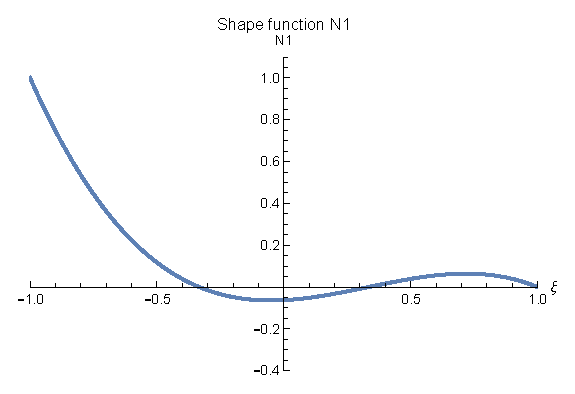
\includegraphics[width=\textwidth]{pdf/shape_function_N1}
    \end{minipage}
    \hfill
    \begin{minipage}[b]{0.45\textwidth}
        \centering
        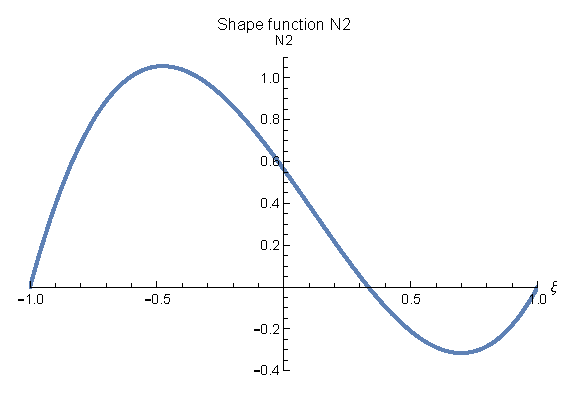
\includegraphics[width=\textwidth]{pdf/shape_function_N2}
    \end{minipage}
    \begin{minipage}[b]{0.45\textwidth}
        \centering
        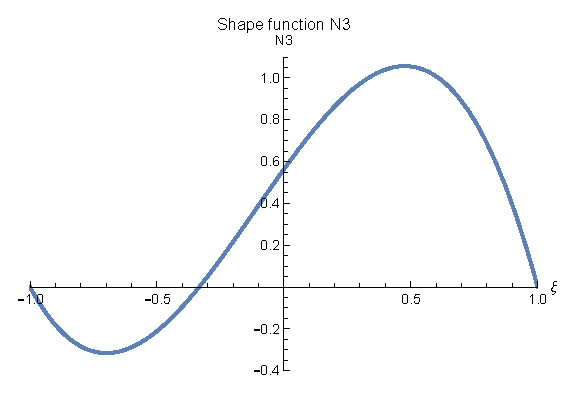
\includegraphics[width=\textwidth]{pdf/shape_function_N3}
    \end{minipage}
    \hfill
    \begin{minipage}[b]{0.45\textwidth}
        \centering
        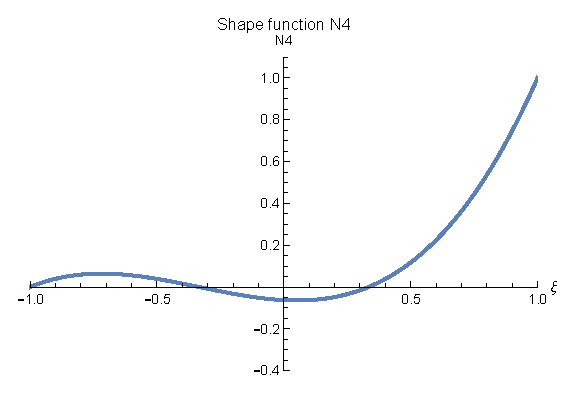
\includegraphics[width=\textwidth]{pdf/shape_function_N4}
    \end{minipage}
    \caption{Shape functions plotted from \texttt{Mathematica}.}
    \label{fig:shape_functions}
\end{figure}

As we know shape functions can also be rearranged in the following matrix form:

\begin{equation}
    \mathbf{N}^e(\xi) = \begin{bmatrix}
        N_1^e(\xi) \quad N_2^e(\xi) \quad N_3^e(\xi) \quad N_4^e(\xi)
    \end{bmatrix}
\end{equation}

\paragraph{Compatibility functions}

During the derivation of the elemental matrices, we will also need to calculate the compatibility functions $B^e(\xi)$.

The compatibility functions are defined as the derivatives of the shape functions with respect to the global coordinates $X$.
Since we have computed the shape functions in terms of the local coordinates $\xi$, we can use both the chain rule and the Jacobian matrix, or perform an inverse mapping from the local to the global coordinates and then differentiate.

\begin{equation}
    B^e(\xi) = \frac{\partial N_i^e(\xi)}{\partial X} =
    \begin{cases}
        \frac{\partial N_i^e(\xi)}{\partial \xi} \frac{\partial \xi}{\partial X}            & \text{using the chain rule}      \\
        \frac{\partial N_i^e(\xi = \xi(X) = \frac{2}{b-a} (X - \frac{a+b}{2}))}{\partial X} & \text{using the inverse mapping}
    \end{cases}
\end{equation}

By adopting one of the two methods above, we can obtain the compatibility functions for the given problem as:

\begin{align}
    B_1^e(\xi) & = \frac{9 \xi (2-3 \xi )+1}{8 h_e}    \\
    B_2^e(\xi) & = \frac{9 (\xi (9 \xi -2)-3)}{8 h_e}  \\
    B_3^e(\xi) & = -\frac{9 (\xi (9 \xi +2)-3)}{8 h_e} \\
    B_4^e(\xi) & = \frac{9 \xi (3 \xi +2)-1}{8 h_e}
\end{align}

In a matrix form, we can write the compatibility functions as:

\begin{equation}
    \mathbf{B}^e(\xi) = \begin{bmatrix}
        B_1^e(\xi) \quad B_2^e(\xi) \quad B_3^e(\xi) \quad B_4^e(\xi)
    \end{bmatrix}
\end{equation}
